\section{Artificial Intelligence}
As mentioned earlier, there is no scripting language in \doom. The A.I. is based on a set of state machines for each enemy type baked into the engine binary. Designers did not have to learn C since they could entirely configure an opponent via the text file \cw{multigen.txt}. This text file is parsed by a tool (cunningly named \cw{multigen}) and compiled into C source code (\cw{info.h} and \cw{info.c}).\\
\par
\rawdrawing{multigen}
\par
% The script has two sections per entity. First the general info and then a serie of state machines. To illustrate here if the imp script.\\
Let's dive into the hand-written state machine descriptor text file right away and take a look at the section of \cw{multigen.txt} that controls the imp (known as \cw{TROOP} internally).\\
\par
\tcode{enemy_info.txt}

\tcode{imp_state.txt}

There are four sections. Properties include the DoomED \cw{id}, \cw{speed}, \cw{height}, \cw{radius}, state names for state machine targets, sound strings, and finally the huge Action definition.






Property lists and sound names are self-explanatory, and there is no need to spend too much time on them. What is more difficult to understand is how the state machine is defined.\\
\par
A thing's state machine is partly statically defined inside the engine (when a monster is attacked it goes directly to \cw{seestate}; when it receives lethal damage, it goes directly to \cw{diestate}) and partly defined in \cw{multigen.txt}. Each line in the state definition follows a syntax:
\begin{enumerate}
\item State name.
\item Frame family.
\item Frame ID (sprite to render).
\item Duration in tics (engine runs 35 tics/second).
\item Function to call when in this state.
\item Next state.
\end{enumerate}
\par
\vspace{5pt}
Let's take the example of an imp that has just spawned in a level and therefore is in state \cw{spawnstate}, which is \cw{S\_TROO\_STND}. Upon entering a state, the engine calls its associated function. In this case, the imp will cycle between the states \cw{S\_TROO\_STND} and \cw{S\_TROO\_STND2}. This means, \cw{A\_Look} is called every 10 tics (roughly 11Hz). If the player is found, \cw{A\_Look} places the imp into the \cw{seestate} (a.k.a S\_TROO\_RUN1).\\
\par

Suppose this imp was unlucky, the player was fast and managed to hit it with a shotgun at point blank. In this case the engine places the imp into the \cw{deathstate} (\cw{S\_TROO\_DIE1}).\\
\par
\tcode{enemy_state_die.txt}\\
\par
Notice how values \cw{I}, \cw{J}, \cw{K}, \cw{L}, and \cw{M} translate to sprite names.\\
\par
\fullimage{imp_die}
\vspace{-10pt}
Let's follow the chain of state from here, where an imp dies in five steps:

\begin{enumerate}
\item Show first death frame (I) for 8/35ths of a second.
\item Show second death frame (J) for 8/35ths of a second. Scream using \cw{deathsound}.
\item Show third death frame (K) for 6/35ths of a second.
\item Show fourth death frame (L) for 6/35ths of a second. Mark itself as non-obstacle (\cw{A\_FALL}).
\item Show fifth death frame (M) forever (\cw{-1}).
\end{enumerate}
\par
The total dying sequence lasts $8+8+6+6=24/35 = 0.68$ seconds. Note that this imp could have been even less lucky and been hit by a rocket. Enough damage would have caused it to gib, moved it to the \cw{xdeathstate} (\cw{S\_TROO\_XDIE1}) state and made it die in $1$ second.\\
\par
\tcode{enemy_state_xdie.txt}\\
\par
\fullimage{imp_xdie}




\par
\begin{wrapfigure}[9]{r}{0.25\textwidth}
\centering

\includegraphics[width=.25\textwidth]{drawings/sprite_quantization.pdf}
\end{wrapfigure}
The engine uses a convention to find which sprite to use when rendering them. Because an enemy will not always be facing the player, it uses quantization where all orientations relative to the player's position fall into eight ranges (see diagram where 1 is facing the player, 5 facing away, and so on).\\
\par
When in the \cw{S\_TROO\_XDIE1} state, according to \cw{multigen.txt}, the engine must use the sprite family \cw{TROO} and frame \cw{N}. Based on the orientation (lets say the imp has its back to the player), the engine should use \cw{TROON5}. However, there is no such sprite in \cw{DOOM.WAD} (exploding enemies always face the player) so the engine falls back to \cw{TROON0} (0 being the "always facing" sprite).\\
\par







\cfullimage{cyber_sprite}{Cyberdemon poses in one of its two "walk" positions.}
\par
Taking a look at one of the frames for the Cyberdemon in figure \ref{cyber_sprite} gives a good idea of the colossal work required from artists. Twelve monsters times eight states times an average of five frames per animation would have required close to 480 drawings (for the monsters only). The power of the NeXTdimension made a tremendous difference in this department.\\
\par
The Cyberdemon however is an extreme case since it is not symmetrical. For the imp, storage is optimized to take advantage of its symmetry. If the engine needs \cw{TROOA6} but doesn't find it in the \cw{WAD}, it uses its opposite (\cw{TROOA4}) and draws it mirrored.\\ 
\par
\trivia{You may have noticed that in the list of states there is a non-obvious one named \cw{RAISE}. This is used when the Arch-Vile resurrects dead monsters. The animation plays the death animation in reverse. Note that there is no reverse gib sequence, but the Arch-Vile still revives gibbed monsters using a reverse normal death animation.}



\begin{figure}[H] \centering
\cscaledimage{0.9}{imp_sprite}{}
\end{figure}
\par
\trivia{When an entity receives more than  \cw{spawnhealth} damage (negative its spawning state; in the case of an imp that would be -60), the engine triggers not \cw{deathstate} but the \cw{xdeathstate} state that means the entity exploded.}\\
\par 
\ccode{explode.c}





\cw{multigen.txt} is compiled to the humongous 5000 line \cw{info.c} containing an array of \cw{state\_t}s holding the state machine, and an array of \cw{mobjinfo\_t}s containing the thing properties.\\
\par
\ccode{enemy_state_compiled.c}\\
\par
\begin{wrapfigure}[9]{r}{0.5\textwidth}
\centering
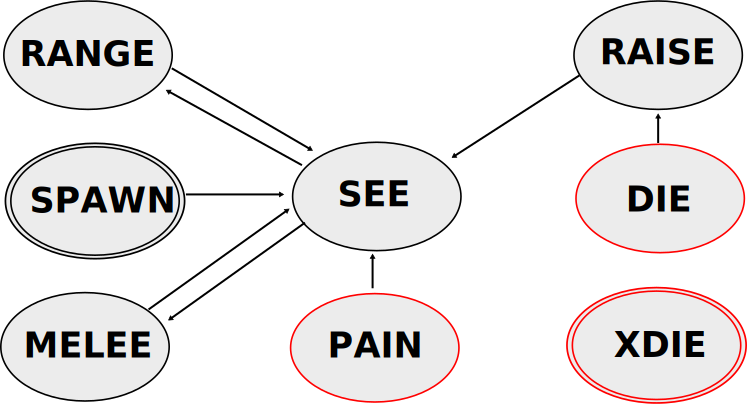
\includegraphics[width=.5\textwidth]{drawings/automate.pdf}
\end{wrapfigure}
Not all automaton state changes can be inferred from the transition array. In the case of the imp, transitions are partly dictated by the logic in \cw{info.txt} (black arrows) and partly dictated by the game engine (direct to red state).\\
\par
 In the state diagram, the engine-triggered transitions to \cw{pain}, \cw{die}, and \cw{xdie} are not represented since these states can be reached directly from any other state.
\par
%In the diagram, note the starting state (\cw{SPAWN}) and the only final state \cw{XDIE}. \cw{DIE} can transition to \cw{RAISE} thanks to the Archville heal power which makes the dead rise. The only way to make sure a monster will never come back is to gib it.

\pagebreak

\subsection{Optimization}
Monsters constantly request collision tests. Even the simple \cw{SPAWN} state, for which a two frame animation cycles repeatedly (monsters do not have a standing script, they "walk on the spot"), calls the \cw{A\_Look} function to attempt to locate the player. Furthermore, once activated, monsters need path-finding and range attack tests. The calculations proved to be an unacceptable level of load on the CPU. Even using the blockmap structure to speed up collision detection it still meant hundreds of rays to cast, thirty five times per second which resulted in thousands of instructions.\\
\par
To solve this problem, another data structure was introduced with \cw{doombsp}. Each sector visibility is precomputed to allow impossible collisions to be rejected early. The visibility data is stored in a bit array\footnote{This approach later morphed into the Potentially Visible Set which was instrumental to Quake engine.}. This dataset is packed into a matrix of size $num\_sectors^2/8$ and stored in a \cw{REJECT} lump. At runtime, the engine compares the player's current sector with a monster's sector to potentially bypass sight detections for this monster entirely.\\
\par
\drawing{reject_explained}{}
% Regardless of the monsters, the base state machine looks like this but it tuned based on custom functions called in some states (e.g: \cw{A\_SpidRefire}, \cw{A\_CyberAttack}, and \cw{A\_BrainExplode}).\\
% \par
% \pngdrawing{automate}{}
\vspace{-7pt}
Figure \ref{reject_explained} features four sectors with five monsters and one player in sector \circled{A}. The engine needs only to run expensive line of sight calculations for the monster in sector \circled{B}. All four others monsters are "rejected" via a cheap lookup. The table is only used for sight. Monsters will still hear the player since sound is cheaper to propagate.\\
\par
\trivia{With "unlimited" CPU power, modern "node builders" don't build \cw{REJECT} anymore.}






\section{Map Intelligence}
Despite lacking a scripting system, maps still managed to offer a rich experience. They were full of surprises with numerous elements interacting with the player. Switches and tripwire-enabled doors, secret passages, elevators, crushing walls, traps and more.\\
\par
\drawing{E1M1_tripwire}{UDOOM's E1M1 features 21 special lines and five of them open secret areas.}
\par
All interactions are achieved via a simple association between a line's \cw{special} attribute which designates one action to perform and a \cw{tag} value that indicates the target sectors to act on.\\
\par
The list of action types is impressive -- there are more than 130 of them: open/close door at normal/turbo/blazing speeds; raise/lower floor and ceilings; fast ceiling crush \& raise; stairbuilders; locked door so you are trapped with monsters; lighting level effects; raise floor to nearest height, texture changes, teleports, level normal and secret exits, and many others.\\
\par
The tag designating the target is any number picked by the designer. Any lines the designer wants to be targeted by this action are tagged with the same number. With this system, a line can trigger only one action but target several sectors.\\
\par
\trivia{The first maps designed had mostly orthogonal walls and military design. It took the team a few months to realize \doom{} engine was capable of much more.}
\pagebreak






\begin{wrapfigure}[17]{r}{0.5\textwidth}
\centering
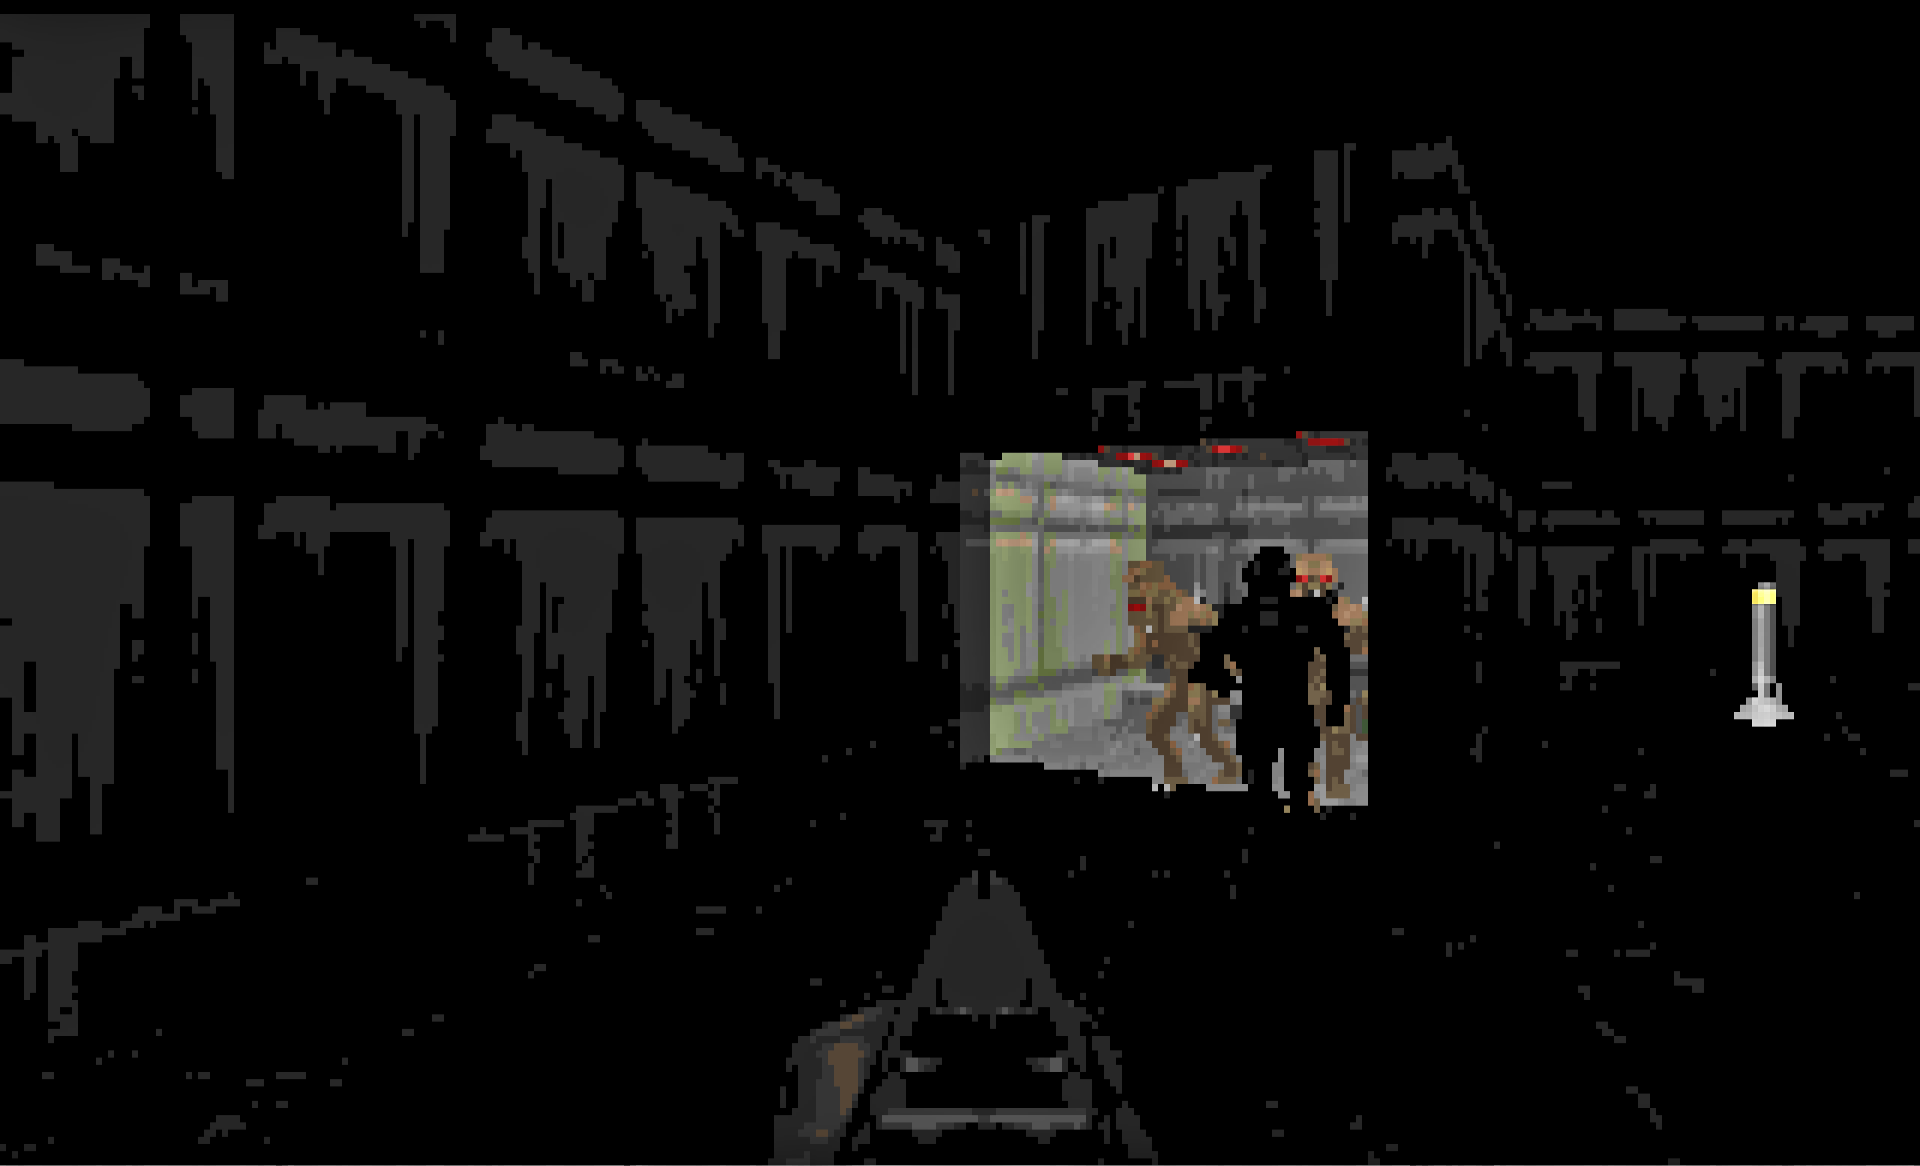
\includegraphics[width=.5\textwidth]{drawings/E1M3_trap.pdf}
\end{wrapfigure}
Who doesn't recognize E1M3's hunt for the blue key on page \pageref{e1m3_trap}? After traversing the whole map, it is finally found sitting on a pedestal, guarded by only two low-level opponents which are easily dispatched.\\
\par
But as soon as the player picks it up, the lights go out and the sound of a door opening and growling imps can be heard. It was a trap the player just walked into and imps are just behind (page \pageref{e1m3_trap})!\\
\par
To implement this effect, two sets of lines were used. The first lines (in blue) target the door sector behind which the monsters were hiding and opens it. The second lines (in red) target the current sector and set its light level to "very dark".\\
\par



\par
\begin{wrapfigure}[23]{l}{0.5\textwidth}
\centering
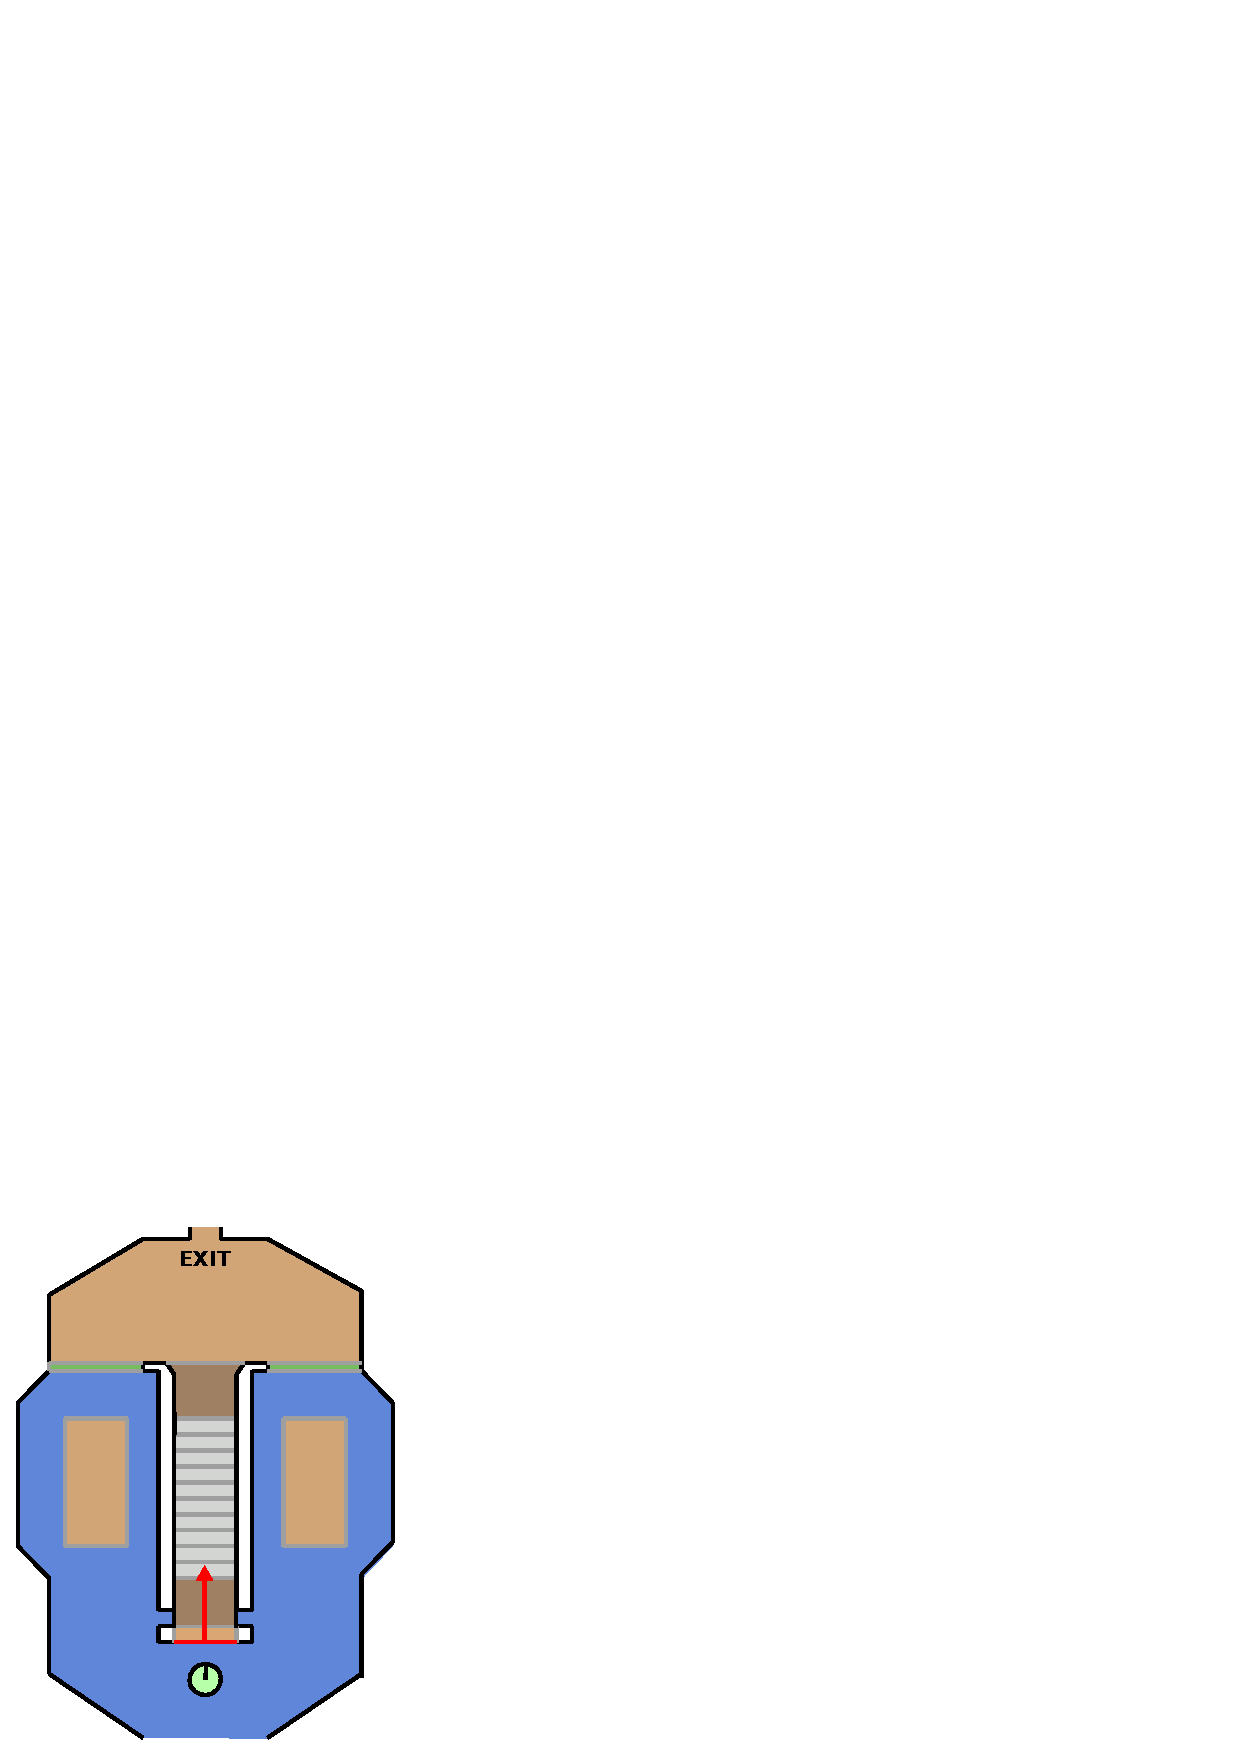
\includegraphics[width=.5\textwidth]{drawings/E1M3_sides2.pdf}
\end{wrapfigure}
Another interesting effect in E1M3 is the rising staircase that leads to a small room containing the exit to level 4. It is implemented by having a line with the "BuildStairs" (\#8) type targeting the first step sector with its tag. The engine has a hardcoded \cw{EV\_BuildStairs} function that looks up the target sector via the tag then uses a flood-fill algorithm.\\
\par Adjacent sectors are repeatedly looked up and a bit more height is added with each iteration. To avoid raising the whole level, the algorithm stops when the next sector's texture is different from the last elevated sector, which explains why the stairs are gray, while the top and bottom surrounding them are dark brown.\\
\par
Before and after screenshots can be seen on page \pageref{stairs}.


\fullimage{Doom-E1M3-Ingame2.png} \label{e1m3_trap} \\
Finally, the blue key (above)! Nooo, it's a TRAP (below)!

\vspace{2mm}
\fullimage{Doom-E1M3-Ingame3.png}
\fullimage{e1m3_after_stairs.png} \label{stairs} \\
Above, all steps start at the same level. Below, after the "BuildStairs" trigger. 

\vspace{2mm}
\fullimage{e1m3_before_stairs.png}



\section{Game Tics Architecture}
With the knowledge of how opponents and map elements work, we can pick up the code where we left it with regard to game simulation on page \pageref{TryRunTics.c}. \cw{G\_Ticker} is where all thinkers are run.\\
\par
\ccode{G_Ticker.c}
\par
Most of the meat is in the 3D gameplay (\cw{P\_Ticker}) function.\\
\par
\ccode{P_Ticker.c}
\par
\cw{P\_PlayerThink} is where the player "thinks". This function consumes the \cw{ticcmd\_t} (which we already studied on page \pageref{cmd_t_type}) and controls where the player moves and fires.\\
\par 
\cw{P\_RunThinkers} is how the map and monsters "think". Anything that must occur over more than one frame is placed in a thinker object and stored in a doubly-linked list. Thinkers are structs with a function pointer and some data for the function pointer parameters. Each gameplay tic, every thinker in the list "thinks". When thinkers are done thinking they set their function pointer to -1 and are dropped from the list. Note that doors have no feelings but they are nonetheless "thinkers" too.\\
\par
\cw{P\_UpdateSpecials} takes care of animating special textures such as water, or animated walls. It also takes care of switching the texture when a button is pushed.\\
\par 

 \cw{P\_RespawnSpecials} respawns medikits, weapons, and ammo in deathmatch.



\ccode{thinker_t.c}\\
\par
C has no OOP capabilities yet the engine managed to implement a polymorphism system. Semantically, \cw{think\_t} structs are stored in the linked list element (\cw{thinker\_t}) with no space for the payload. \\%But since all thinkers start with a function pointer, the engine stores the function pointer and the data parameter payload with a single pointer. \\
\par
\ccode{floormove_t.c}\\
\par
\cw{EV\_BuildStairs}, which creates thinkers to build stairs, shows how to use the system.\\
\par
\ccode{EV_BuildStairs.c}\\
\par
This is a pretty cool mechanism. While iterating over the list of \cw{thinker\_t}, the loop simply calls \cw{thinker->function(thinker)} which has no knowledge of either the function called or the payload involved.
